\documentclass{beamer}
\usepackage[utf8]{inputenc}
\usepackage[brazil]{babel}
\usepackage[T1]{fontenc}
\usepackage{graphicx}
\usepackage{calc}
\usepackage{enumitem}

\title{Um conto sobre softwares}
\author{João G. Santos}

\usetheme{Berkeley}

\begin{document}
\maketitle

\begin{frame}
  \frametitle{Modelo tradicional}
  Historicamente as aplicações web foram construídas da seguinte maneira, graças à influência de linguagens procedurais como PHP e ASP clássico.

  \vspace{1.5\baselineskip}
  \begin{itemize}
    \item Programação procedural ou mista
    \item Código maior e menos legível
    \item Maior propensão a comportamentos inesperados (bugs)
  \end{itemize}
\end{frame}

\begin{frame}
  \frametitle{O porco de 127 quilos}
  \begin{center}
    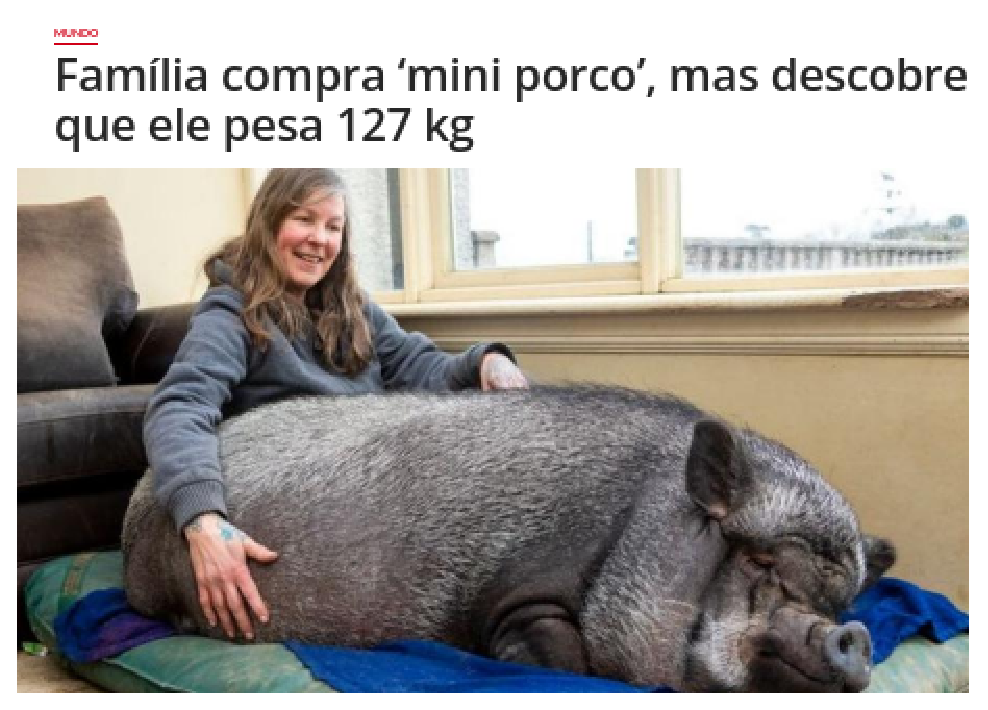
\includegraphics[width=\linewidth-12ex]{porco.eps}
  \end{center}
\end{frame}

\begin{frame}
  \frametitle{Modelo escalável}
  Para solucionar o problema do software que precisa crescer sem se tornar gradativamente imprevisível e complexo, os engenheiros de software contemporâneos adotaram convenções que visam tornar a base de código \textit{escalável} (leia-se: apta a incrementação).

  \vspace{1.5\baselineskip}
  \begin{itemize}
    \item Programação estritamente orientada a objetos
    \item Código suscinto e legível
    \item Centenas ou milhares de linhas de código reaproveitadas
  \end{itemize}
\end{frame}

\begin{frame}
  \frametitle{Porque isso interessa a empresa}
  \begin{itemize}
    \item Velocidade para implementar funcionalidades
    \item Código mais seguro (menos código significa menos bugs)
    \item Facilita o entendimento por novos membros da equipe
  \end{itemize}
  
  \vspace{1.5\baselineskip}
  O sistema pode ser incrementado \textit{ad infinitum} sem se tornar um caos e o código final se torna mais seguro, robusto e auditável. Todos ganham com isso.
\end{frame}

\begin{frame}
  \frametitle{Como seria o ERP ideal da Capsul?}
  \begin{description}[style=nextline,itemsep=2ex]
    \item[Divisão em camadas] Permite que eventualmente profissionais qualificados sejam designados para postos específicos\pause
    \item[Integração contínua (CI)] Funcionalidades são adicionadas sob demanda sem interromper o sistema em produção\pause
    \item[Acompanhamento direto] Feedback e solicações feitas diretamente para a equipe interna da empresa
  \end{description}
\end{frame}

\begin{frame}
  \frametitle{Como seria o ERP ideal da Capsul?}
  \begin{center}
  \textbf{E por último\ldots}
  \end{center}\pause

  \vspace{1.5\baselineskip}
  \begin{description}[style=nextline]
    \item[Fortalece a informatização da empresa] O software é construído de modo escopado e dedicado, sem a dependência de terceiros e em contato direto com os líderes
  \end{description}
\end{frame}
\end{document}
